

Our task is to design a framework for end-to-end text streams multi-classification that is able to overcome the challenges mentioned above. We assume that there are two types of input stream elements: labeled and unlabeled texts. Every text has a unique identifier. The framework should predict and deliver labels for raw texts, while labeled ones must be used for additional training. In section~\ref{DSP}, we introduce a processing engine used for computations and explain the rationale behind the choice. Data flow and its properties are explained in detail in~\ref{DF}. We touch upon the ML model that can be applied to the task in~\ref{ML}.

\begin{figure}[htbp]
  \centering
  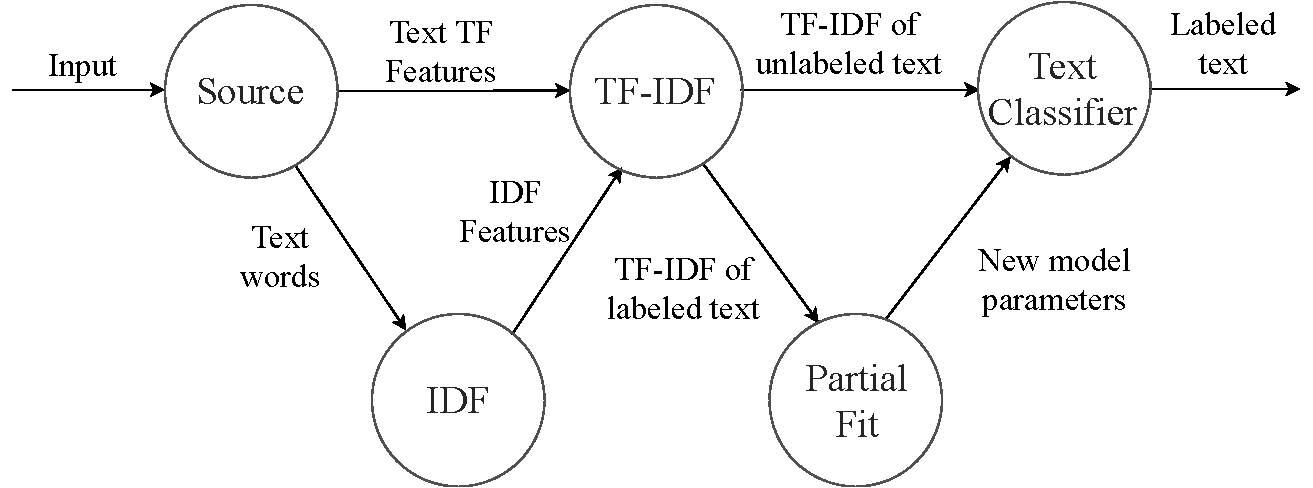
\includegraphics[scale=0.48]{pics/logical-graph}
  \caption{The logical pipeline}
  \label {logical_graph}
\end{figure}

\subsection{Distributed stream processing\label{DSP}}

In order to process high-velocity data at scale, the stream processing systems are commonly used as a solution. The examples of such systems are Apache Flink~\cite{Carbone:2017:SMA:3137765.3137777}, Google's MillWheel~\cite{Akidau:2013:MFS:2536222.2536229}, Spark Streaming~\cite{Zaharia:2012:DSE:2342763.2342773}, and Apache Storm~\cite{apache:storm}. In these systems, every piece of data enters and exits the system one by one or within small-sized blocks. Inside a system, elements are also transformed independently from each other or with slight buffering, e.g. within time windows. Unlike batch-processing systems, the next processing stages do not wait until previous ones are completed. 

For scalability, these systems are running on clusters of computers. Calculations are evenly distributed among all computers. Usually, each operation in a data flow has a user-defined balancing function for determining the shard where an element will be processed. That is, after each transformation every element can be sent to another machine using this scheme. For example, for distributed IDF processing the function should send the same words to the same shard.

Such computational model provides low latency between an input element arrival and the delivery of results, however, it is hard to provide consistency guarantees on data in case of failures. Most of the stream processing systems have a lack of determinism, which means that the result of computing is not the same between independent launches. Hence, it is challenging to create a stable framework with testing and validating final results as it was discussed in~\cite{stonebraker20058}. Another issue is connected with the exactly-once delivery guarantee. This guarantee ensures processing of each element by exactly one time. Batch-processing systems provide full fault tolerance and consistency, however in stream processing exactly-once is a challenging problem that solved with big overhead. This affects the latency and makes it less than one second~\cite{S7530084, we2018beyondmr} which is commonly unacceptable.

In this work, our computations based on~\FlameStream\ ~\cite{we2018beyondmr} distributed engine, which provides the following advantages:

\textbf{Determinism.} Results are determined only by input and remain the same between independent runs.

\textbf{Exactly-once.} Process data in an exactly-once manner by default, which the same data processing on the Spark systems, for example, will be at a worse performance.

The mentioned problems are solved in~\FlameStream\ with almost no overhead. This allows us to create a classifier with predictable results and due to the exactly-once delivery guarantee provide low latency.

\subsection{Data flow \label{DF}}

\subsubsection{Computational pipeline}

Similar to other stream processing systems,~\FlameStream\ sets scheme of calculations by a logical directed graph. Every vertex in the graph represents a transform operation. An oriented edge indicates the flow and kind of data.

For our task, the calculations can be illustrated as a logical graph illustrated in Figure~\ref{logical_graph}. Input vertex receives incoming texts, calculates term frequencies and transfers them to the {\em TF-IDF} vertex. It also sends words from the text to {\em IDF} vertex. {\em IDF} computes the inverse frequency of the words and delivers them to the {\em TF-IDF} vertex. {\em TF-IDF} joins corresponding inverse documents frequencies together with term frequencies within a given text. After that, the complete {\em TF-IDF} features are sent to {\em Text Classifier} vertex. {\em Text Classifier} predicts the label and delivers the result to the user.

\begin{figure}[htbp]
  \centering
  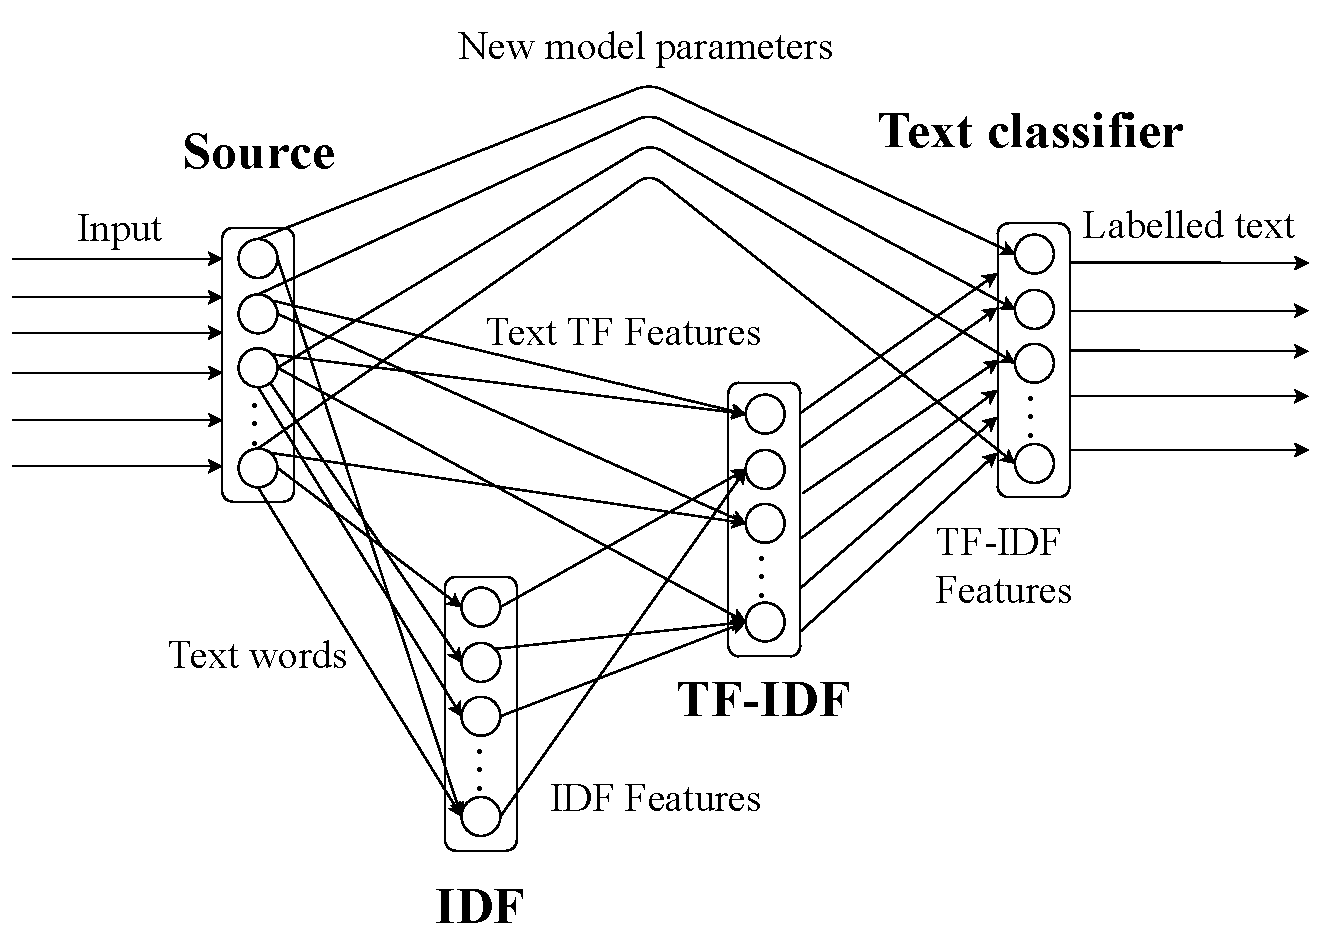
\includegraphics[scale=0.375]{pics/physical-graph}
  \caption{The physical pipeline}
  \label {physical_graph}
\end{figure}

When the pipeline is deployed, the logical graph maps into a physical graph(Figure ~\ref{physical_graph}). Each logical task is mapped to a number of physical tasks. This is, every vertex here is a single computational unit. Each rectangle denotes the same cluster of computers.

Input texts are received by all machines. Shuffle before {\em IDF} vertex are defined by a hash function of a word. Partitioning before {\em TF-IDF} physical vertices are determined by a text id. There is no network shuffle between {\em TF-IDF} and {\em Text Classifier} vertices, so they are simply chained. The {\em Partial Fit} operation is located on a single machine and broadcasts model parameters to {\em Text Classifier} vertices.

\subsubsection{Dealing with concept drift}

Concept drift is a phenomenon of changing users' interests from time to time, which usually depends on recent events, and results in shifting the distribution of text classes to particular ones. Essentially, this may affect the correctness of the pipeline, more specifically, the computing of the IDF features. To overcome the issue, we use windowed IDF calculation: concrete IDF values will be provided based on input within a time window. For instance, the window can be set to a day or a week. This scheme allows us to deal with sudden changes in the topics. Similar approaches are applied in [?].

\subsubsection{Partial fit}

Figures ~\ref{logical_graph}, ~\ref{physical_graph} provide a scheme for a partial fitting. Labeled input documents accumulate in the Partial Fit vertex. Additional training is triggered by a special element, which is submitted to the input as an ordinary element. However, this element is not processed as a text and the vertices just push the element further. This process is similar to punctuation processing \cite{tucker2003exploiting}. The conditions, when the partial fitting starts, can be chosen arbitrarily by a system administrator. For example, one can update machine learning model on every 1000 labeled documents.

\subsection{ML model \label{ML}}

The classifier's model can be chosen independently from other computations. In our case, we use Multinomial Logistic Regression. At the start of the system, the initial classifier parameters such as weights can be provided by a pre-train process.

Every time, when the Partial Fit is triggered, the following process occurs, which can be described in terms of the optimization of a cost function. This function in our case is written below:

\begin{center}

$$ J(W) = -\frac{1}{m} \sum \limits_{i = 1}^{m} \sum \limits_{j = 1}^{k} \mathbbm{1}_{\left\{y^{(i)} == j\right\}} \cdot \log \frac{\exp\left({W_{j}^Tx^{(i)}}\right) }{\sum \limits_{l = 1}^{k}  \exp\left({W_{l}^Tx^{(i)}}\right) }$$ 
 $$ +  \lambda_1 ||W||_1 + \lambda_2 ||W - W_{prev}||_2 $$

\end{center} 

The number of points in a new dataset is denoted as $m$. The point with index $i$ showed as $x^{(i)}$. The number of classes is $k$. New weights are designated as $W$. The weights, that computed in the previous step, are $W_{prev}$. At the first time of triggering the process, $W_{prev}$ are the pre-trained weights. 

The formula provides the goal of the training. The first component is the standard softmax function for multiple classes. The second component keeps the l1 regularization of the weights. The important aspect is the regularization provides sparsity, hence, the model has a small size -- about 1 Mb, which can be stored and updated with low cost. To use the previous history of the classifier weights we apply l2 regularization as the third component. Fitting new points and the consideration of the previous weights ensure better accuracy of the classifier.

We are interested in finding such $W$ that minimizes $J(W)$. Taking derivatives, one can show that the gradient for each class component is:

\begin{center}

$$ \nabla_{W_j} \; J(W) = -\frac{1}{m} \sum \limits_{i = 1}^{m} \left[ x^{(i)} \left( \mathbbm{1}_{\left\{y^{(i)} == j\right\} } - \frac{\exp\left({W_{j}^Tx^{(i)}}\right)}{\sum \limits_{l = 1}^{k}  \exp\left({W_{l}^Tx^{(i)}}\right)} \right) \right] $$
$$ - \; \lambda_1 sign\left(W\right) - \frac{\lambda_2}{2} \left(W - W_{prev} \right), \; j = [1..k] $$

\end{center} 

We use Stochastic Gradient Descent for optimization. In experiments ~\ref{fs-short-experiments} section, model performance is presented.